\documentclass{article}
\usepackage{amsmath}
\usepackage{amssymb}
\usepackage{graphicx}
\usepackage{hyperref}
\usepackage[version=4]{mhchem}


\begin{document}
\(A B C D\) is a convex quadrilateral. \(A B=C D \neq A D . M\) and \(N\) are midpoints of \(A D, B C\), respectively. Connect \(M N\). Which one of the following is true?\\
(A) \(A B=M N\)\\
(B) \(A B>M N\)\\
(C) \(A B<M N\)\\
(D) All could be true.\\
\centering
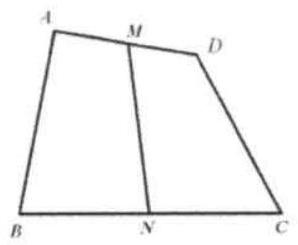
\includegraphics[width=\textwidth]{images/038.jpg}

Solution: (B).\\
Connect \(A C\). Take \(P\), the midpoint of \(A C\). Connect \(P A, P N\). Since \(M\) and \(P\) are midpoints of \(A D, A C\), respectively, by Theorem 2.1,

\[
M P=\frac{1}{2} D C
\]

Since \(N\) and \(P\) are midpoints of \(B C, A C\), respectively, by Theorem 2.1,

\[
\begin{aligned}
& N P=\frac{1}{2} A B \\
& (1)+(2): M P+N P=\frac{1}{2} D C+\frac{1}{2} A B
\end{aligned}
\]

We know that \(A B=C D\).\\
\centering
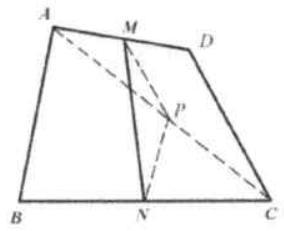
\includegraphics[width=\textwidth]{images/038(3).jpg}\\
(3) can be written as \(M P+N P=A B\)

By the triangle inequality theorem, \(M P+N P>M N\).\\
Thus \(A B>M N\)


\end{document}
